\documentclass{standalone}
\usepackage{tikz}
\usepackage{amsmath,amssymb,amsthm,mathtools}

\usetikzlibrary{3d,arrows.meta}
\usetikzlibrary{matrix, positioning}

\begin{document}

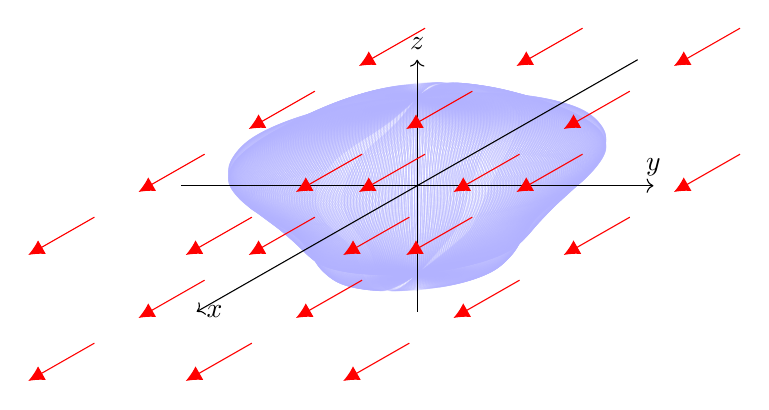
\begin{tikzpicture}[scale=2,
        x={(-0.7cm,-0.4cm)},
        y={(1cm,0cm)},
        z={(0cm,0.8cm)}]

    \foreach \t in {0,1,...,350} {
            \draw[blue!30,opacity=0.4]
            plot[smooth cycle,samples=36,variable=\s,domain=0:360]
            ({0.6*cos(\s)*(1+0.2*sin(3*\s))*cos(\t)},
            {cos(\s)*(1+0.2*sin(3*\s))*sin(\t)},
            {0.7*sin(\s)*(1+0.1*sin(4*\s))});
        }

    \draw[->] (-2,0,0) -- (2,0,0) node[right] {$x$};
    \draw[->] (0,-1.5,0) -- (0,1.5,0) node[above] {$y$};
    \draw[->] (0,0,-1) -- (0,0,1) node[above] {$z$};

    \foreach \x in {-1.5,-0.5,0.5,1.5}
    \foreach \y in {-1,0,1}
    \foreach \z in {-0.5,0.5}
    \draw[-{Latex[length=2mm,width=2mm]},red] (\x,\y,\z) -- ++(0.6,0,0);
\end{tikzpicture}

\end{document}